% Options for packages loaded elsewhere
\PassOptionsToPackage{unicode}{hyperref}
\PassOptionsToPackage{hyphens}{url}
\PassOptionsToPackage{dvipsnames,svgnames,x11names}{xcolor}
%
\documentclass[
  letterpaper,
  DIV=11,
  numbers=noendperiod]{scrreprt}

\usepackage{amsmath,amssymb}
\usepackage{iftex}
\ifPDFTeX
  \usepackage[T1]{fontenc}
  \usepackage[utf8]{inputenc}
  \usepackage{textcomp} % provide euro and other symbols
\else % if luatex or xetex
  \usepackage{unicode-math}
  \defaultfontfeatures{Scale=MatchLowercase}
  \defaultfontfeatures[\rmfamily]{Ligatures=TeX,Scale=1}
\fi
\usepackage{lmodern}
\ifPDFTeX\else  
    % xetex/luatex font selection
\fi
% Use upquote if available, for straight quotes in verbatim environments
\IfFileExists{upquote.sty}{\usepackage{upquote}}{}
\IfFileExists{microtype.sty}{% use microtype if available
  \usepackage[]{microtype}
  \UseMicrotypeSet[protrusion]{basicmath} % disable protrusion for tt fonts
}{}
\makeatletter
\@ifundefined{KOMAClassName}{% if non-KOMA class
  \IfFileExists{parskip.sty}{%
    \usepackage{parskip}
  }{% else
    \setlength{\parindent}{0pt}
    \setlength{\parskip}{6pt plus 2pt minus 1pt}}
}{% if KOMA class
  \KOMAoptions{parskip=half}}
\makeatother
\usepackage{xcolor}
\setlength{\emergencystretch}{3em} % prevent overfull lines
\setcounter{secnumdepth}{5}
% Make \paragraph and \subparagraph free-standing
\ifx\paragraph\undefined\else
  \let\oldparagraph\paragraph
  \renewcommand{\paragraph}[1]{\oldparagraph{#1}\mbox{}}
\fi
\ifx\subparagraph\undefined\else
  \let\oldsubparagraph\subparagraph
  \renewcommand{\subparagraph}[1]{\oldsubparagraph{#1}\mbox{}}
\fi

\usepackage{color}
\usepackage{fancyvrb}
\newcommand{\VerbBar}{|}
\newcommand{\VERB}{\Verb[commandchars=\\\{\}]}
\DefineVerbatimEnvironment{Highlighting}{Verbatim}{commandchars=\\\{\}}
% Add ',fontsize=\small' for more characters per line
\usepackage{framed}
\definecolor{shadecolor}{RGB}{241,243,245}
\newenvironment{Shaded}{\begin{snugshade}}{\end{snugshade}}
\newcommand{\AlertTok}[1]{\textcolor[rgb]{0.68,0.00,0.00}{#1}}
\newcommand{\AnnotationTok}[1]{\textcolor[rgb]{0.37,0.37,0.37}{#1}}
\newcommand{\AttributeTok}[1]{\textcolor[rgb]{0.40,0.45,0.13}{#1}}
\newcommand{\BaseNTok}[1]{\textcolor[rgb]{0.68,0.00,0.00}{#1}}
\newcommand{\BuiltInTok}[1]{\textcolor[rgb]{0.00,0.23,0.31}{#1}}
\newcommand{\CharTok}[1]{\textcolor[rgb]{0.13,0.47,0.30}{#1}}
\newcommand{\CommentTok}[1]{\textcolor[rgb]{0.37,0.37,0.37}{#1}}
\newcommand{\CommentVarTok}[1]{\textcolor[rgb]{0.37,0.37,0.37}{\textit{#1}}}
\newcommand{\ConstantTok}[1]{\textcolor[rgb]{0.56,0.35,0.01}{#1}}
\newcommand{\ControlFlowTok}[1]{\textcolor[rgb]{0.00,0.23,0.31}{#1}}
\newcommand{\DataTypeTok}[1]{\textcolor[rgb]{0.68,0.00,0.00}{#1}}
\newcommand{\DecValTok}[1]{\textcolor[rgb]{0.68,0.00,0.00}{#1}}
\newcommand{\DocumentationTok}[1]{\textcolor[rgb]{0.37,0.37,0.37}{\textit{#1}}}
\newcommand{\ErrorTok}[1]{\textcolor[rgb]{0.68,0.00,0.00}{#1}}
\newcommand{\ExtensionTok}[1]{\textcolor[rgb]{0.00,0.23,0.31}{#1}}
\newcommand{\FloatTok}[1]{\textcolor[rgb]{0.68,0.00,0.00}{#1}}
\newcommand{\FunctionTok}[1]{\textcolor[rgb]{0.28,0.35,0.67}{#1}}
\newcommand{\ImportTok}[1]{\textcolor[rgb]{0.00,0.46,0.62}{#1}}
\newcommand{\InformationTok}[1]{\textcolor[rgb]{0.37,0.37,0.37}{#1}}
\newcommand{\KeywordTok}[1]{\textcolor[rgb]{0.00,0.23,0.31}{#1}}
\newcommand{\NormalTok}[1]{\textcolor[rgb]{0.00,0.23,0.31}{#1}}
\newcommand{\OperatorTok}[1]{\textcolor[rgb]{0.37,0.37,0.37}{#1}}
\newcommand{\OtherTok}[1]{\textcolor[rgb]{0.00,0.23,0.31}{#1}}
\newcommand{\PreprocessorTok}[1]{\textcolor[rgb]{0.68,0.00,0.00}{#1}}
\newcommand{\RegionMarkerTok}[1]{\textcolor[rgb]{0.00,0.23,0.31}{#1}}
\newcommand{\SpecialCharTok}[1]{\textcolor[rgb]{0.37,0.37,0.37}{#1}}
\newcommand{\SpecialStringTok}[1]{\textcolor[rgb]{0.13,0.47,0.30}{#1}}
\newcommand{\StringTok}[1]{\textcolor[rgb]{0.13,0.47,0.30}{#1}}
\newcommand{\VariableTok}[1]{\textcolor[rgb]{0.07,0.07,0.07}{#1}}
\newcommand{\VerbatimStringTok}[1]{\textcolor[rgb]{0.13,0.47,0.30}{#1}}
\newcommand{\WarningTok}[1]{\textcolor[rgb]{0.37,0.37,0.37}{\textit{#1}}}

\providecommand{\tightlist}{%
  \setlength{\itemsep}{0pt}\setlength{\parskip}{0pt}}\usepackage{longtable,booktabs,array}
\usepackage{calc} % for calculating minipage widths
% Correct order of tables after \paragraph or \subparagraph
\usepackage{etoolbox}
\makeatletter
\patchcmd\longtable{\par}{\if@noskipsec\mbox{}\fi\par}{}{}
\makeatother
% Allow footnotes in longtable head/foot
\IfFileExists{footnotehyper.sty}{\usepackage{footnotehyper}}{\usepackage{footnote}}
\makesavenoteenv{longtable}
\usepackage{graphicx}
\makeatletter
\def\maxwidth{\ifdim\Gin@nat@width>\linewidth\linewidth\else\Gin@nat@width\fi}
\def\maxheight{\ifdim\Gin@nat@height>\textheight\textheight\else\Gin@nat@height\fi}
\makeatother
% Scale images if necessary, so that they will not overflow the page
% margins by default, and it is still possible to overwrite the defaults
% using explicit options in \includegraphics[width, height, ...]{}
\setkeys{Gin}{width=\maxwidth,height=\maxheight,keepaspectratio}
% Set default figure placement to htbp
\makeatletter
\def\fps@figure{htbp}
\makeatother

\KOMAoption{captions}{tableheading}
\makeatletter
\makeatother
\makeatletter
\@ifpackageloaded{bookmark}{}{\usepackage{bookmark}}
\makeatother
\makeatletter
\@ifpackageloaded{caption}{}{\usepackage{caption}}
\AtBeginDocument{%
\ifdefined\contentsname
  \renewcommand*\contentsname{Tabla de contenido}
\else
  \newcommand\contentsname{Tabla de contenido}
\fi
\ifdefined\listfigurename
  \renewcommand*\listfigurename{List of Figures}
\else
  \newcommand\listfigurename{List of Figures}
\fi
\ifdefined\listtablename
  \renewcommand*\listtablename{List of Tables}
\else
  \newcommand\listtablename{List of Tables}
\fi
\ifdefined\figurename
  \renewcommand*\figurename{Figure}
\else
  \newcommand\figurename{Figure}
\fi
\ifdefined\tablename
  \renewcommand*\tablename{Table}
\else
  \newcommand\tablename{Table}
\fi
}
\@ifpackageloaded{float}{}{\usepackage{float}}
\floatstyle{ruled}
\@ifundefined{c@chapter}{\newfloat{codelisting}{h}{lop}}{\newfloat{codelisting}{h}{lop}[chapter]}
\floatname{codelisting}{Listing}
\newcommand*\listoflistings{\listof{codelisting}{List of Listings}}
\makeatother
\makeatletter
\@ifpackageloaded{caption}{}{\usepackage{caption}}
\@ifpackageloaded{subcaption}{}{\usepackage{subcaption}}
\makeatother
\makeatletter
\@ifpackageloaded{tcolorbox}{}{\usepackage[skins,breakable]{tcolorbox}}
\makeatother
\makeatletter
\@ifundefined{shadecolor}{\definecolor{shadecolor}{rgb}{.97, .97, .97}}
\makeatother
\makeatletter
\makeatother
\makeatletter
\makeatother
\ifLuaTeX
  \usepackage{selnolig}  % disable illegal ligatures
\fi
\IfFileExists{bookmark.sty}{\usepackage{bookmark}}{\usepackage{hyperref}}
\IfFileExists{xurl.sty}{\usepackage{xurl}}{} % add URL line breaks if available
\urlstyle{same} % disable monospaced font for URLs
\hypersetup{
  pdftitle={Semestre 2023-2},
  pdfauthor={Carlos Mario Castaño},
  colorlinks=true,
  linkcolor={blue},
  filecolor={Maroon},
  citecolor={Blue},
  urlcolor={Blue},
  pdfcreator={LaTeX via pandoc}}

\title{Semestre 2023-2}
\author{Carlos Mario Castaño}
\date{01-8-2023}

\begin{document}
\maketitle
\ifdefined\Shaded\renewenvironment{Shaded}{\begin{tcolorbox}[boxrule=0pt, breakable, interior hidden, borderline west={3pt}{0pt}{shadecolor}, sharp corners, enhanced, frame hidden]}{\end{tcolorbox}}\fi

\renewcommand*\contentsname{Tabla de contenido}
{
\hypersetup{linkcolor=}
\setcounter{tocdepth}{2}
\tableofcontents
}
\bookmarksetup{startatroot}

\hypertarget{portada}{%
\chapter*{Portada}\label{portada}}
\addcontentsline{toc}{chapter}{Portada}

\markboth{Portada}{Portada}

Aquí se alojara todo lo correspondiente al semestre 2023-2 cursado en la
Universidad Nacional de Colombia.

En la imagen de portada: \textbf{Manami} de \emph{Yowamushi pedal.}

\part{Series de tiempo}

\hypertarget{introducciuxf3n}{%
\chapter{Introducción}\label{introducciuxf3n}}

esto es series de tiempo!

\part{Métodos no paramétricos}

\hypertarget{estimaciuxf3n-histograma-de-la-densidad}{%
\chapter{Estimación histograma de la
densidad}\label{estimaciuxf3n-histograma-de-la-densidad}}

\newcommand{\lr}[1]{\left(#1\right)}
\newcommand{\var}[1]{\textrm{Var}\left[#1\right]}
\newcommand{\esp}[1]{\textrm{E}\left[#1\right]}
\newcommand{\rm}[1]{\textrm{#1}}

La idea es que una variable aleatoria tiene un proceso o función de
densidad subyacente la cuál genera los datos que tendremos finalmente a
disposición. Dada una variable aleatoria \(X\), entonces
\(X \sim f\left(x;\theta\right)\). En el caso paramétrico la estimación
de la función de densidad estaría dada por
\(\hat f \left(x;\theta\right) = f\left(x;\hat{\theta}\right)\)
asumiendo que la población de la cuál provienen los datos sigue una
distribución conocida con función de densidad \(f\).

En el caso no paramétrico, no se hace supuesto alguno sobre la función
de densidad asociada a la población de la cuál provienen los datos. La
estimación de la función de densidad puede hacerse por diferentes
métodos, entre ellos los siguientes:

\begin{itemize}
\tightlist
\item
  Histograma
\item
  Polígono de frecuencias
\item
  Núcleo (kernel)
\end{itemize}

El primer enfonque es realizar la estimación de la función de densidad
usando la \textbf{estimación histograma de la densidad}. Por ejemplo, si
se tienen 100 datos cuyo histograma de frecuencias absolutas está dado
por:

\begin{Shaded}
\begin{Highlighting}[]
\NormalTok{x }\OtherTok{\textless{}{-}} \FunctionTok{rnorm}\NormalTok{(}\DecValTok{100}\NormalTok{, }\DecValTok{0}\NormalTok{, }\DecValTok{1}\NormalTok{)}
\FunctionTok{hist}\NormalTok{(x, }\AttributeTok{freq=}\ConstantTok{TRUE}\NormalTok{, }\AttributeTok{col =} \StringTok{"\#42A5F5"}\NormalTok{)}
\end{Highlighting}
\end{Shaded}

\begin{figure}[H]

{\centering 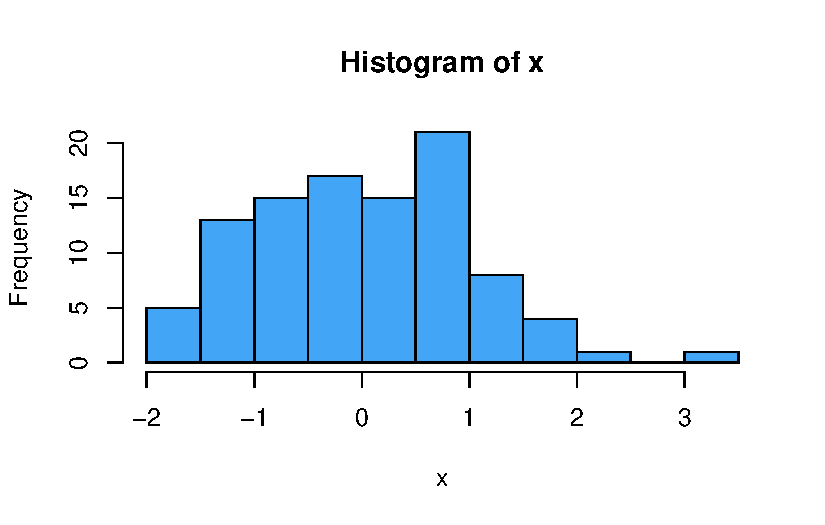
\includegraphics{capitulos/nopara1_files/figure-pdf/unnamed-chunk-1-1.pdf}

}

\end{figure}

La estimación histograma de la densidad dados estos 100 datos es el
siguiente:

\begin{Shaded}
\begin{Highlighting}[]
\FunctionTok{hist}\NormalTok{(x, }\AttributeTok{freq=}\ConstantTok{FALSE}\NormalTok{, }\AttributeTok{col =} \StringTok{"\#42A5F5"}\NormalTok{)}
\end{Highlighting}
\end{Shaded}

\begin{figure}[H]

{\centering 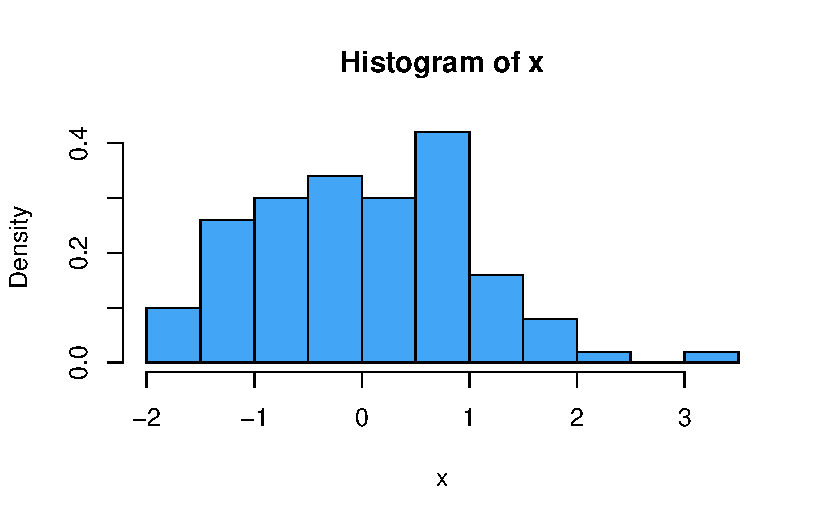
\includegraphics{capitulos/nopara1_files/figure-pdf/unnamed-chunk-2-1.pdf}

}

\end{figure}

Para realizar la estimación se tiene en cuenta lo siguiente:

\begin{itemize}
\tightlist
\item
  \(f\left(x\right)\) es la función de densidad asociada a la variable
  aleatoria \(X\)
\item
  \(\hat{f}\left(x\right)\) es la estimación de la función de densidad
\item
  \(\hat f_H \left(x\right)\) es la estimación histograma de la función
  de densidad
\item
  El área de cada rectángulo del histograma se denota por \(f_j\) y
  depende del número de datos cuyo valor cae en el dicho intervalo y del
  número total de datos, de tal manera que \(f_j = \frac{n_j}{n}\)
\item
  El área de cada rectángulo también puede verse en términos de la
  estimación histograma y de la amplitud del intervalo.
  \(\hat{f}_H \left(x\right) \times 2b\) donde \(b\) es un valor a la
  derecha y a la izquierda del centro del intervalo.
\end{itemize}

Así, se tiene que si la amplitud del intervalo es \(2b\), entonces:

\[\frac{n_j}{n} = 2b \hat{f}_H \left(x\right)\]
\[\hat{f}_H \left(x\right)=\frac{n_j}{2nb} \hspace{0.5cm} \textrm{donde} \hspace{0.5cm} n_j=\sum_{i=1}^n \mathbf{I}_{\left[x-b, x+b\right]} \left(x_i\right)\]
Ahora, según \(n_j\) se tiene que:

\[ 
\begin{align}
x-b \leq x_i \leq x+&b\\
-b \leq x_i-x \leq &b\\
-1 \leq \frac{x_i-x}{b} \leq 1
\end{align}
\] y por lo tanto

\[n_j = \sum_{i=1}^n \mathbf{I}_{\left[-1,1\right]}\left(\frac{x_i-x}{b}\right)\]

luego, la estimación histograma de la densidad puede escribirse como:

\[\hat{f}_H \left(x\right) = \frac{1}{nb} \sum_{i=1}^n \frac{1}{2} \mathbf{I}_{\left[-1,1\right]}\left(\frac{x_i-x}{b}\right) = \frac{1}{nb} \sum_{i=1}^n K_U\left(u\right)\]
donde

\[u = \left(\frac{x_i-x}{b}\right) \hspace{0.5cm} \mathrm{y} \hspace{0.5cm} K_U\left(u\right) = \begin{cases}\frac{1}{2} & -1<u<1 \\ 0 & \text { e.o.c }\end{cases}\]
\(K_U\) es un kernel uniforme. Es decir, es una función de densidad
centrada en \(0\) y toma valores de la forma \(u\) entre \(-1\) y \(1\).

Si ahora se supone que la amplitud del intervalo es \(b\), entonces se
tiene que:

\[\frac{n_j}{n} = b\hat{f}_H \left(x\right)\]
\[\hat{f}_H \left(x\right)=\frac{n_j}{nb} \hspace{0.5cm} \textrm{donde} \hspace{0.5cm} n_j=\sum_{i=1}^n \mathbf{I}_{\left[x-\frac{b}{2}, x+\frac{b}{2}\right]} \left(x_i\right)\]
de \(n_j\) se tiene que

\[ 
\begin{align}
x-\frac{b}{2} \leq x_i \leq x+&\frac{b}{2}\\
-\frac{b}{2} \leq x_i-x \leq &\frac{b}{2}\\
-\frac{1}{2} \leq \frac{x_i-x}{b} \leq &\frac{1}{2}
\end{align}
\] y por lo tanto:

\[\hat{f}_H \left(x\right)=\frac{1}{nb} \sum_{i=1}^n \mathbf{I}_{\left[-\frac{1}{2},\frac{1}{2}\right]}\left(\frac{x_i-x}{b}\right)=\frac{1}{nb}K_U\left(u\right)\]
donde

\[u = \left(\frac{x_i-x}{b}\right) \hspace{0.5cm} \mathrm{y} \hspace{0.5cm} K_U\left(u\right) = \begin{cases} 1 & -\frac{1}{2}<u<\frac{1}{2} \\ 0 & \text { e.o.c }\end{cases}\]
en forma general, si la amplitud del intervalo es \(ab\) entonces:

\[\hat{f}_H \left(x\right)=\frac{1}{nb} \sum_{i=1}^n \frac{1}{a} \mathbf{I}_{\left[-\frac{ab}{2},\frac{ab}{2}\right]}\left(\frac{x_i-x}{b}\right)=\frac{1}{nb}K_U\left(u\right)\]
donde

\[u = \left(\frac{x_i-x}{b}\right) \hspace{0.5cm} \mathrm{y} \hspace{0.5cm} K_U\left(u\right) = \begin{cases} \frac{1}{a} & -\frac{ab}{2}<u<\frac{ab}{2} \\ 0 & \text { e.o.c }\end{cases}\]

\hypertarget{propiedades-del-estimador-histograma}{%
\section{Propiedades del estimador
histograma}\label{propiedades-del-estimador-histograma}}

Dado que el estimador histograma de la densidad depende de la amplitud
\(b\) del intervalo, la idea es escoger el valor de la amplitud que
minimice el \(\textrm{MSE}\) para así poder encontrar una estimación más
exacta de la función de densidad subyacente a la población en cuestión.

\begin{align}
\textrm{Var}\left[\hat b - b\right] &= \textrm{E}\left[\left(\hat b - b\right)^2\right] - \left(\textrm{E}\left[\hat b - b\right]\right)^2\\
\textrm{Var}\left[\hat b\right] &= \underbrace{\textrm{E}\left[\left(\hat b - b\right)^2\right]}_{\textrm{MSE}} - \underbrace{\left(\textrm{E}\left[\hat b\right]-b\right)^2}_{\textrm{BIAS}^2}\\
\end{align}

y despejando, se tiene que:

\[\underbrace{\textrm{E}\left[\left(\hat b - b\right)^2\right]}_{\textrm{MSE}} = \textrm{Var}\left[\hat b\right] + \underbrace{\left(\textrm{E}\left[\hat b\right]-b\right)^2}_{\textrm{BIAS}^2}\]

\part{Bases de datos}

\hypertarget{introducciuxf3n-1}{%
\chapter{Introducción}\label{introducciuxf3n-1}}



\end{document}
